\section{Introduction}\label{sec:introduction}
 \textit{Bidirectional transformation} (denoted by "bx") is a technique used to synchronize two (or more) instance of different meta-models. Both models are related, but don't necessarily contain the same information. Changes in one model thus lead to changes in the other model \cite{bx-grace}. Bx makes sure that two models that can change over time have to be kept constantly consistent with each other.
\newline\newline\textit{Bidirectional transformation} is used to deal with scenarios like:
\begin{itemize}
	\item {change propagation to the user interface as a result of underlying data changes}	
	\item {synchronization of business/software models}
	\item {refreshable data-cache incase of database changes}
	\item {consistency management between two artifacts by avoiding data loss}
\end{itemize}
    and many more....

\subsection{Contribution}\label{subsec:contribution}    
Bx community has been doing research and development work in many fields like software development, database, mathematics and much more to increase awareness and to reach more people \cite{bx-dagstuhl}\cite{bx-grace}. As a result, many kinds of bx tools are being developed, e.g., eMoflon \cite{emoflon-part4}, Echo \cite{echo}. These bx tools are based on various approaches, such as graph transformations, bidirectionalization, update propagations \cite{bx-community} and can be used in different areas of application.

\subsection{Problem Statement}\label{subsec:probstmt}
\textit{Bidirectional transformation} is an emerging concept. In the past, many efforts have been made by conducting international workshops, seminars and through experiments conducted by developers / bx community to identify its potential. Also, in addition to the development of bx tools and bx language, benchmarks are being created for bx tools for systematic comparison \cite{benchmark-BX}.
\newline\newline  Although a significant amount of work has been done in this field, some basic problems still remain:
\begin{itemize}
	\item {Reachability to relevant communities is not significant due to the absence of a common vocabulary for bx across research disciplines \cite{bx-theoryandappl}. Seminars are still conducted for exchanging ideas in different communities to define a common vocabulary of terms and properties for bx \cite{bx-dagstuhl}.}	
	\item {Bx tools and their applicability is still not widely known even in the developers' communities. Due to the existing conceptual and practical challenges associated with configuring/trying a bx-tool for knowing its potential, using bx, bx-tools in building software systems, many developers and researchers are still using non-bx transformation tools to achieve properties which can be easily supported by bx-tools \cite{bx-theoryandappl}.}
	\item {Absence of a simple yet interactive bx tool demonstrator to depict the potential of \textit{bidirectional transformation} over preferred non-bx tool demonstrators among developers' and researchers' communities \cite{bx-theoryandappl}.}
\end{itemize}

\subsection{Solution Strategy}\label{subsec:solution}
To solve the problems as described in Section \ref{subsec:probstmt}, in this thesis, my goals are as follows:
\begin{itemize} 
\item {Design and implement an interactive demonstrator.} 
\item {Spreading the basic concepts of bx to a wide audience and making them accessible and understandable.}
\end{itemize}
An existing bx tool will be used as a part of the demonstrator to realize \textit{bidirectional transformation}. The final prototype will be interactive and easily accessible to users to help them understand the potential, power and limitations of bx.

\subsection{Structure}\label{subsec:structure}
This document is structured as follows: 

Chapter 1 (introduction) contains the introduction and motivation about the thesis with a solution strategy.

Chapter 2 discusses the related terminologies with respect to bidirectional transformation.

Chapter 3 describes the related work that has been done on bx in last few years and the related problems.

Chapter 4 explains the research work that I have done throughout my thesis along with research questions that I aimed at solving with my work.

Chapter 5 describes all the high-level concepts of my implementation work in brief with related diagrams.

Chapter 6 provides the in-depth details of each implementation layer along with UML diagrams.

Chapter 7 presents a walkthrough of the application from UI perspective.

Chapter 8 contains the feedback from user groups, evaluation results and learning goals(based on research questions).

Chapter 9 contains the feedback from user groups, evaluation results and learning goals(based on research questions).

Last chapter summarizes all the work which was done as part of this thesis and draws useful conclusions followed by future work.

\section{Foundation}\label{sec:foundation}
In this chapter, I am going to describe some commonly used terminologies with respect to bx so that the reader doesn't have any problem in understanding the further chapters.

As already mentioned, "bx is a technique to maintain consistency(synchronize) between two(or more) related models".

\paragraph{Model}is an artefact or external representation of reality which reflects certain relevant aspects of a real system. It is denoted as "M".
\begin{itemize}
\item {Artefact, because it is something artificial, not real.}
\item {External representation, because it can be a drawing, a physical object or software generated on a computer.}
\item {Certain relevant aspects, because it contains some properties related to the real system.}
\end{itemize}
\paragraph{State} denotes the condition of an artefact at any given point of time.
\paragraph{Transformation} is the process in which an artefact undergo a change from one state to another. It is denoted as "X". Refer Figure~\ref{fig:Transformation_Diagram}.
\begin{figure}
	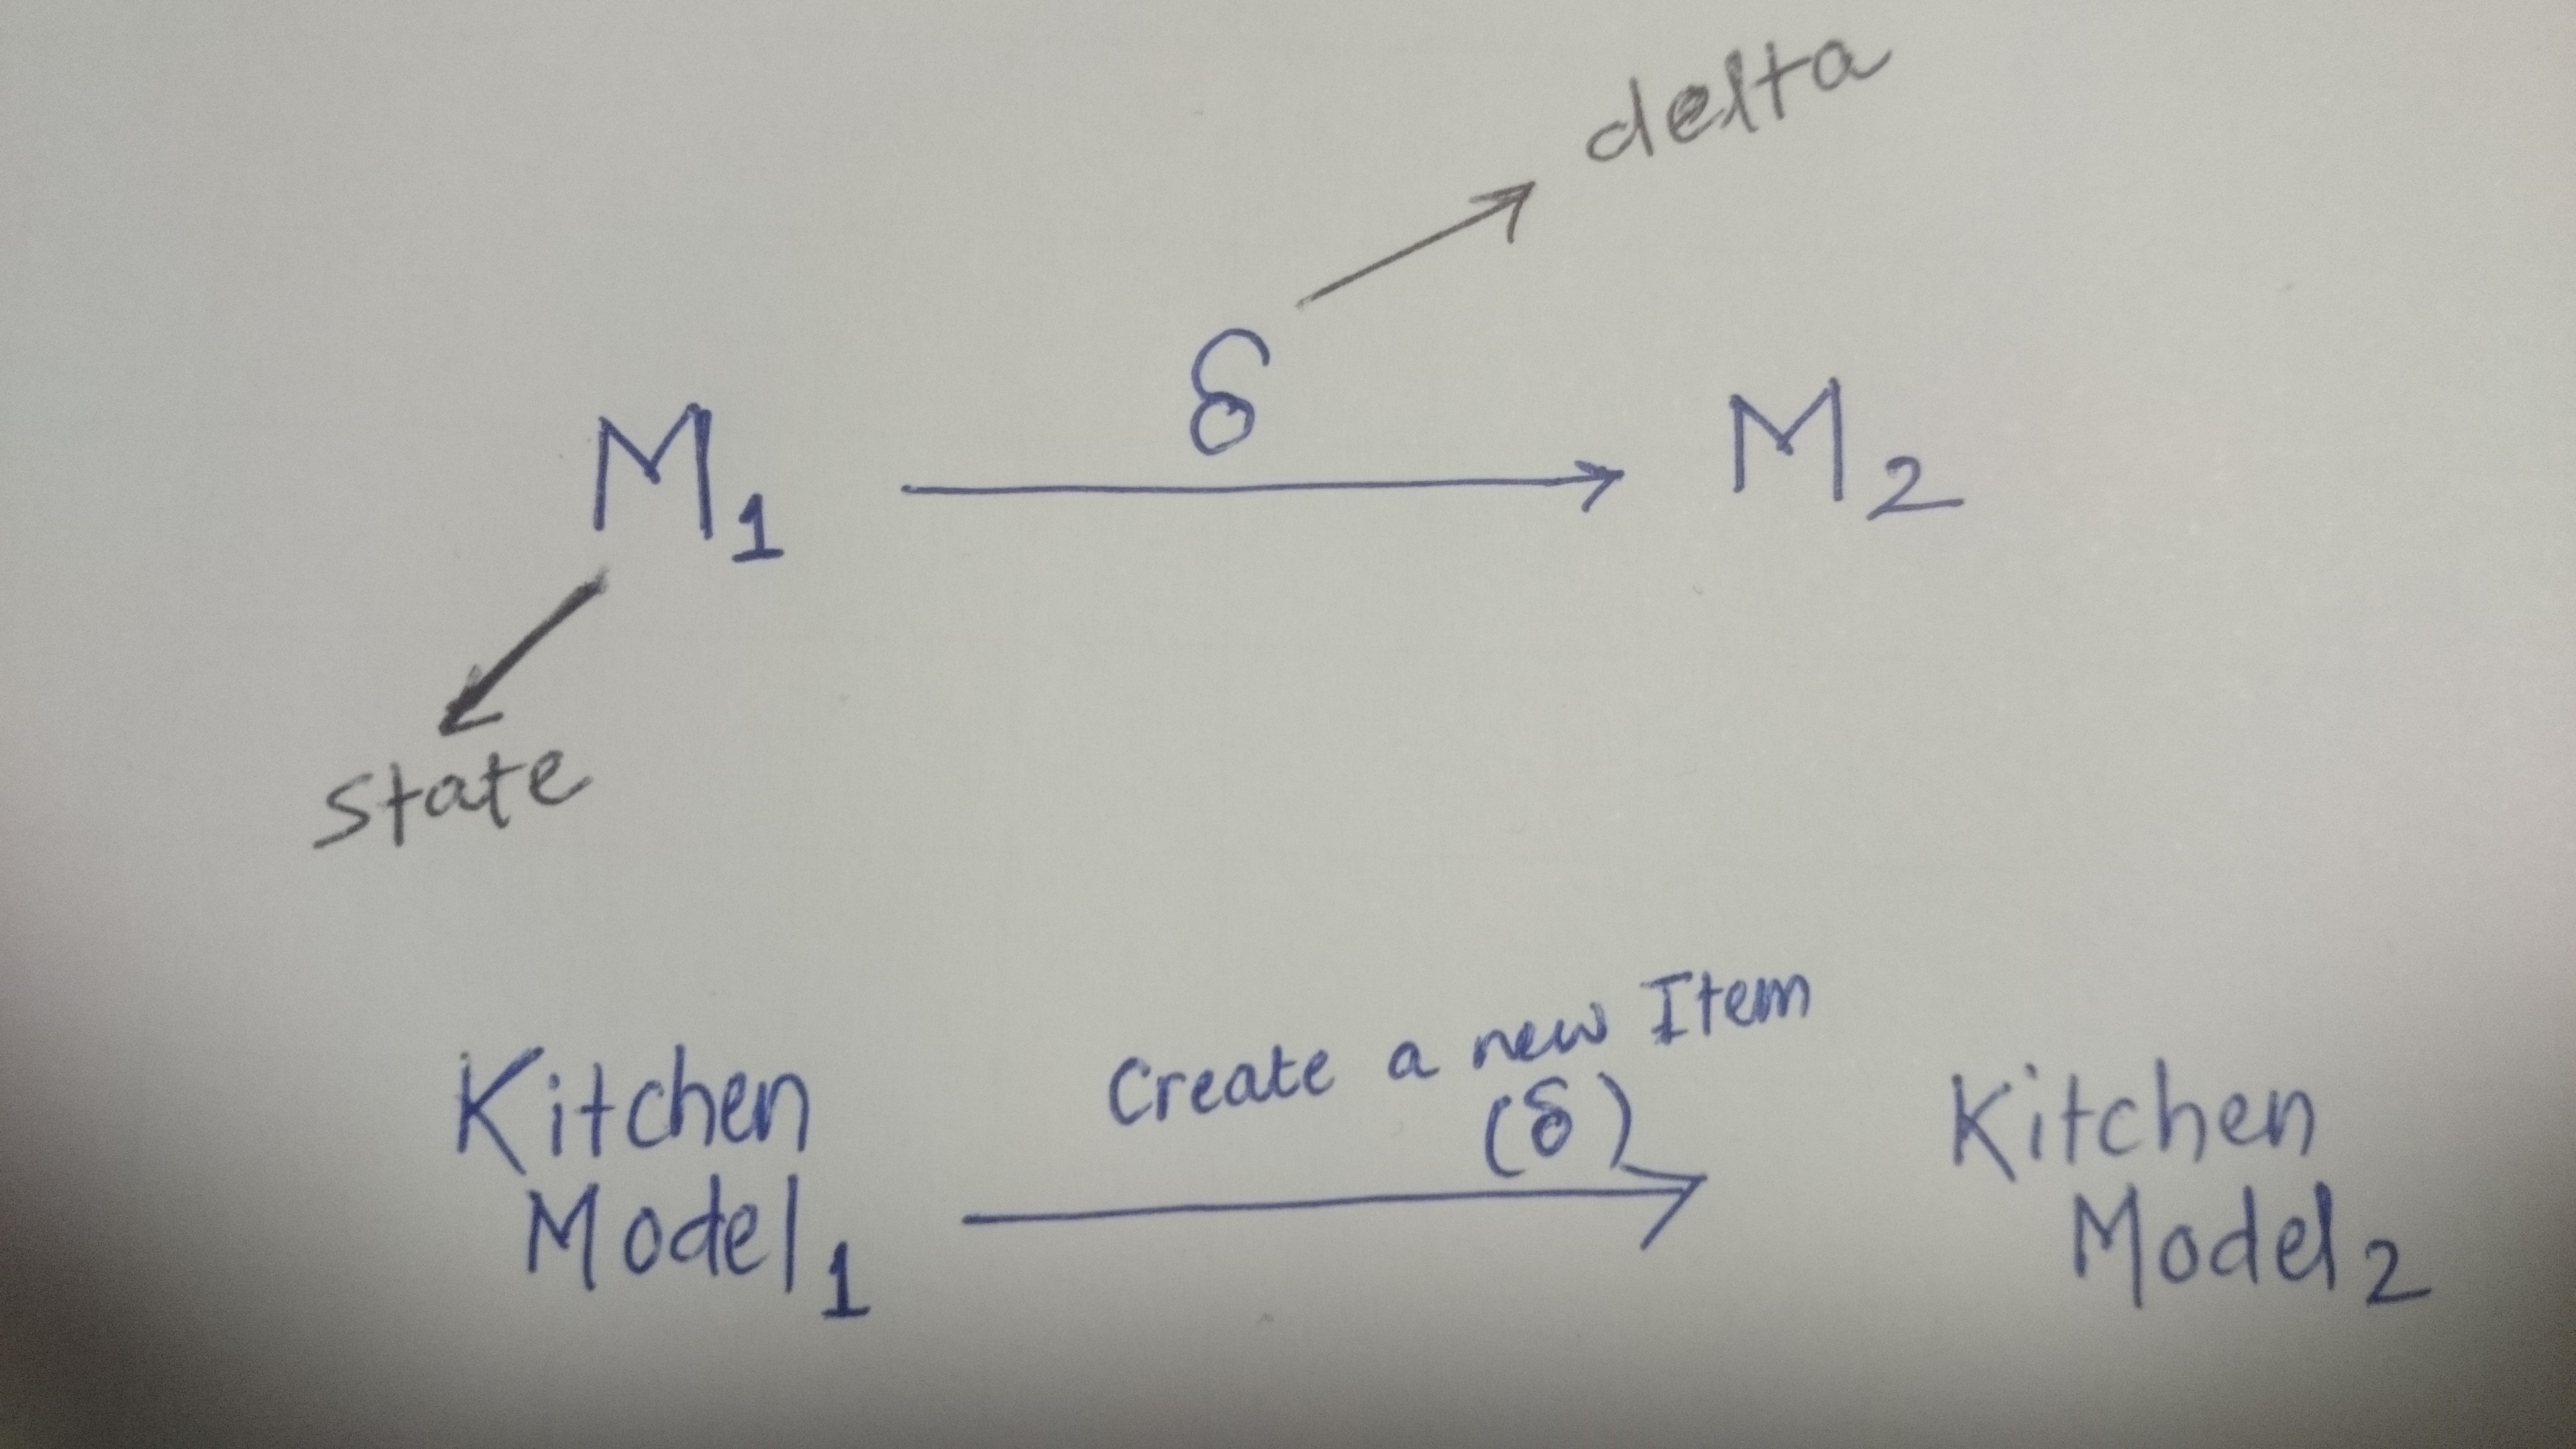
\includegraphics[width=1\textwidth]{figures/Transformation}
	\caption{Transformation}
	\label{fig:Transformation_Diagram}
\end{figure}
\paragraph{Delta} is the change done to one or more properties of an artefact which causes the transformation (X). It is denoted as $\delta$.
\paragraph{State Space} describes all the states of an artefact and all the deltas which lead from one state to another. Refer Figure~\ref{fig:StateSpace_Diagram}.
\begin{figure}
	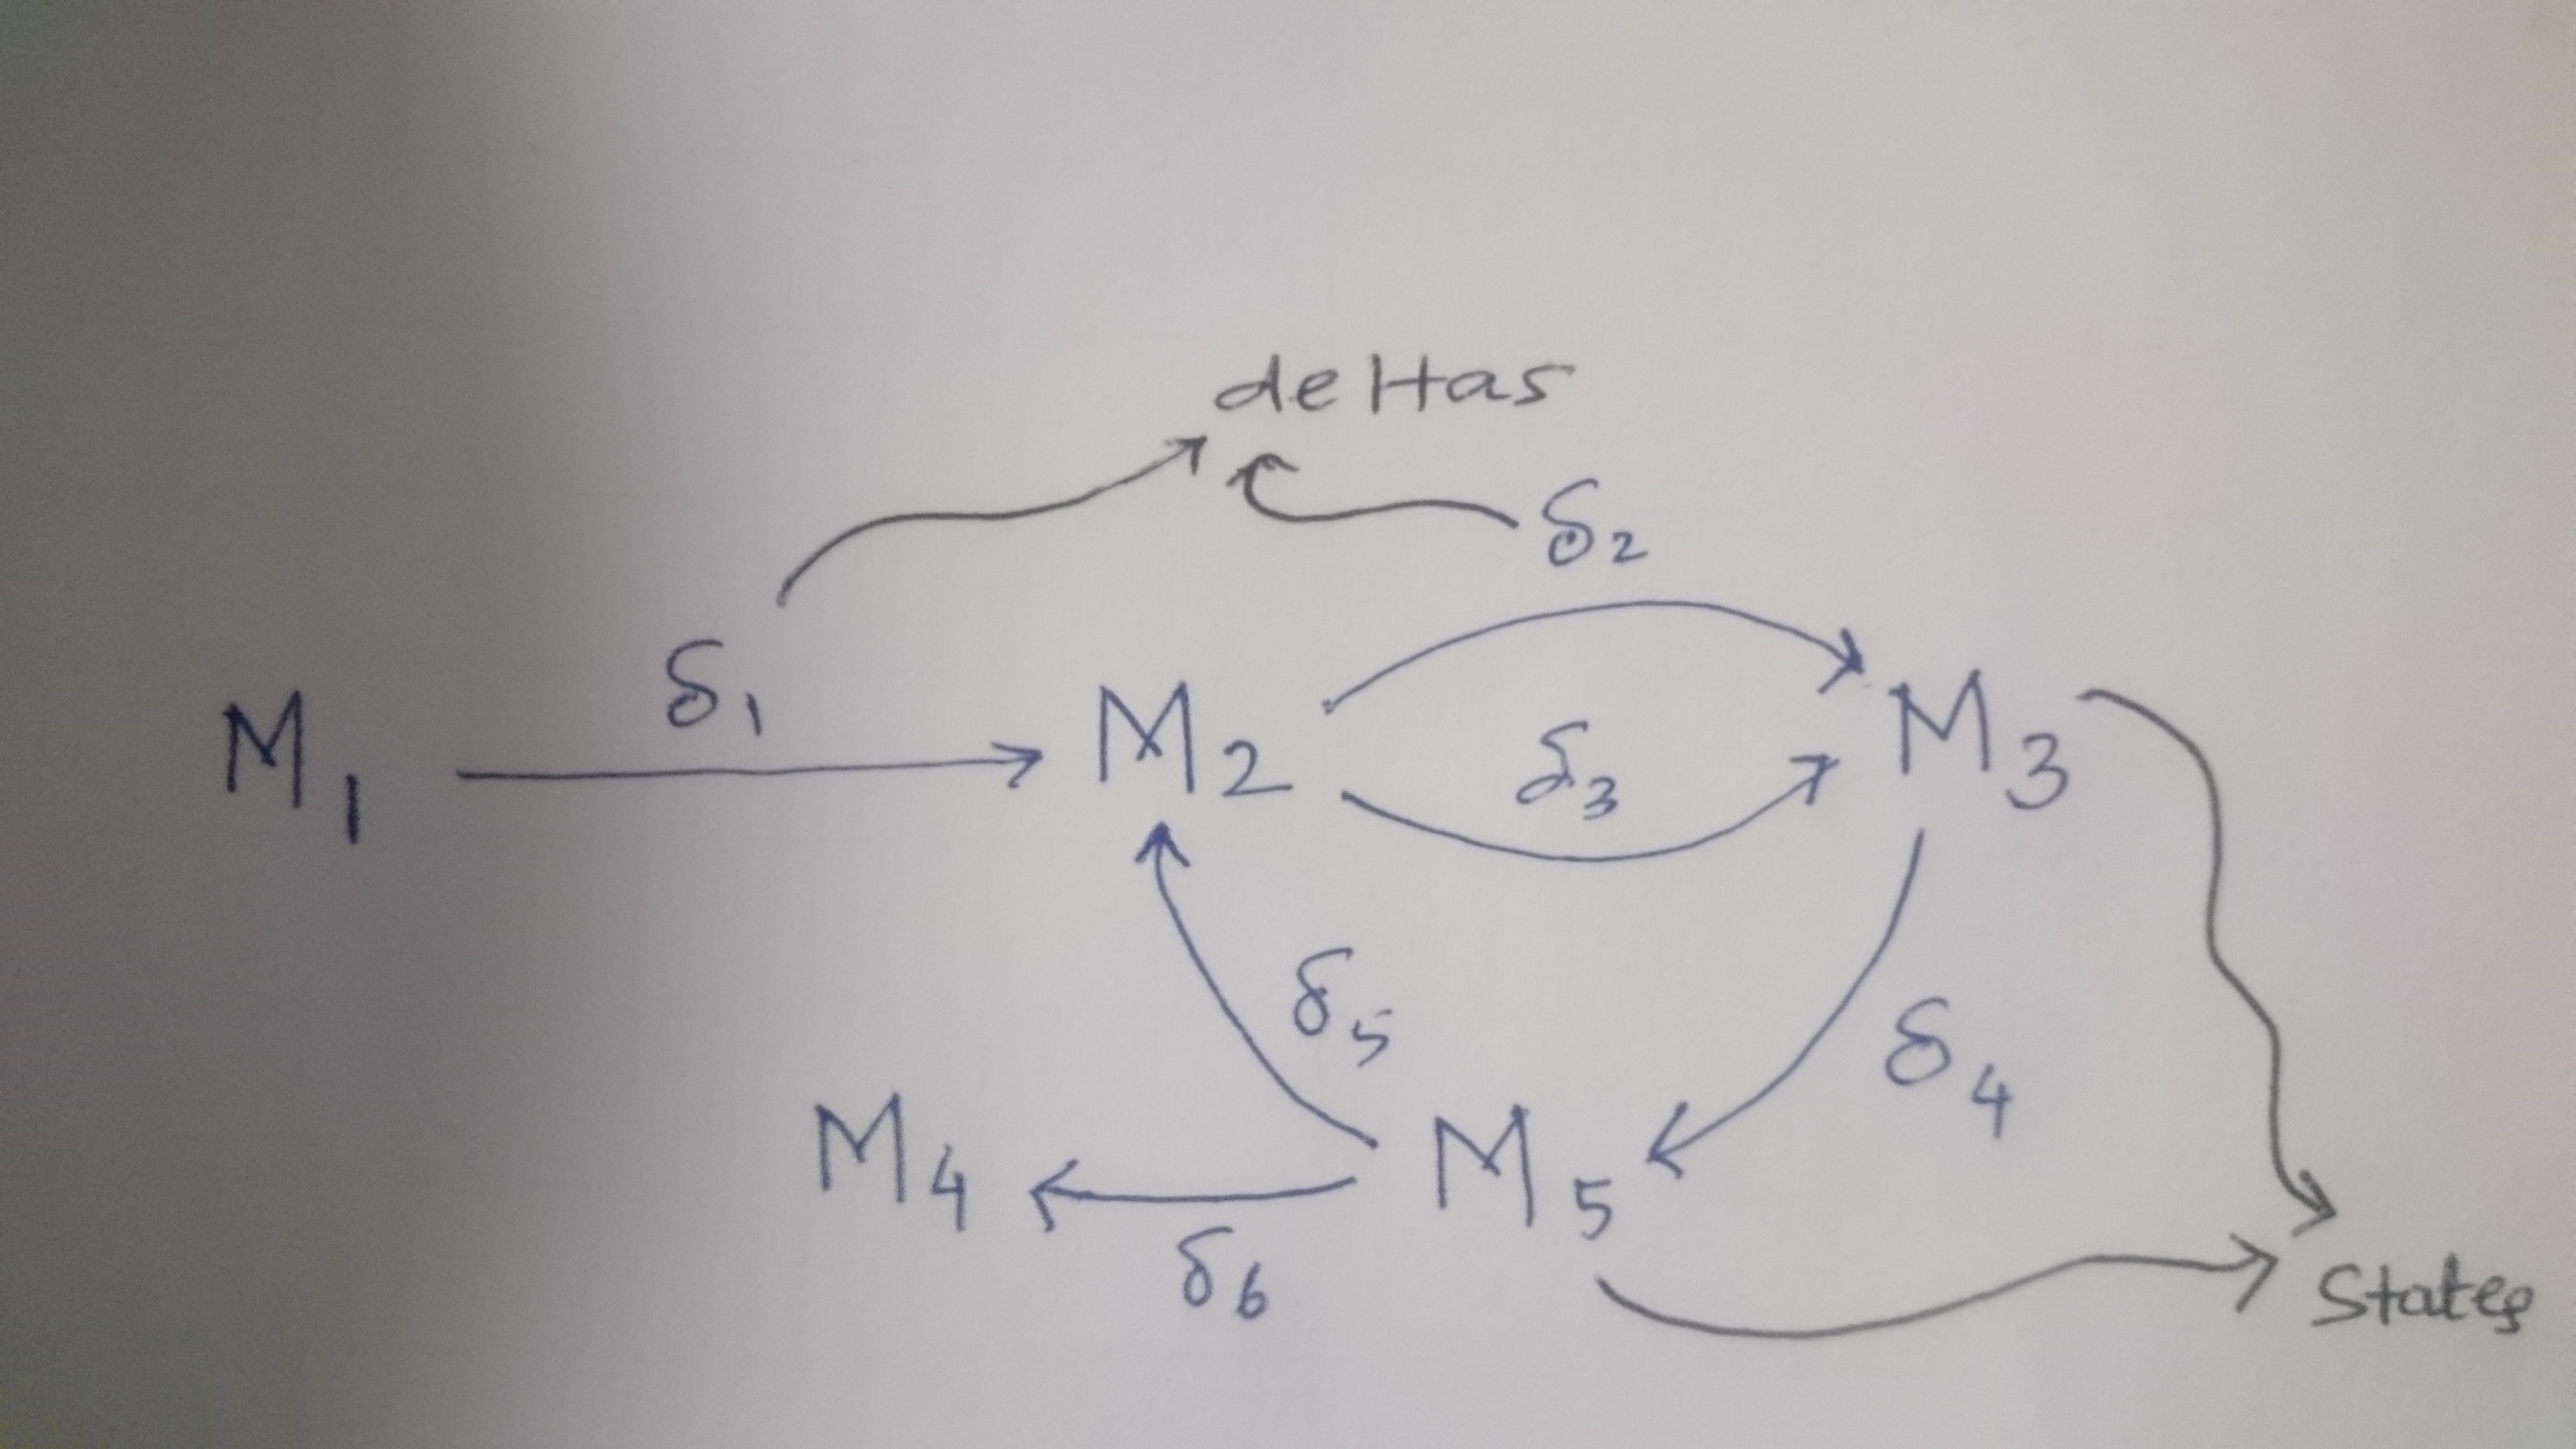
\includegraphics[width=1\textwidth]{figures/State_Space}
	\caption{State Space}
	\label{fig:StateSpace_Diagram}
\end{figure}
\paragraph{Consistency} In layman's term, consistent is a state which always involves 2 or more objects/artefacts but doesn't involve ambiguity between them. This is the most important part of the model transformation and the entire focus revolves around it. To be consistent with each other the models have to be inline with respect to their states. Changes in one model may or may not cause any change in other model but their states must not contain any contradiction. In model-transformation , the most important part is to 
\paragraph{Unidirectional vs.Bidirectional Transformation}  Unidirectional is the simplest one out of all kinds of transformation. It always takes one type of input and produces same type of output \cite{wiki-transformation}. The concept of consistency is very simple as the input model is consistent with the output model, only.
\newline Whereas, bidirectional transformationis a pair of transformation which takes place in both forward and backward direction. One model can be input sometimes and output at some other time. The concept of consistency is relatively complex as more than one model and the models must be kept consistent. Source model ($M_{S}$) is transformed to target model ($M_{T}$) in forward transformation and vice-versa in backward transformation. It is denoted by "BX". 
\newline Figure~\ref{fig:BX_Diagram} describes the concept in detail.
\begin{figure}
	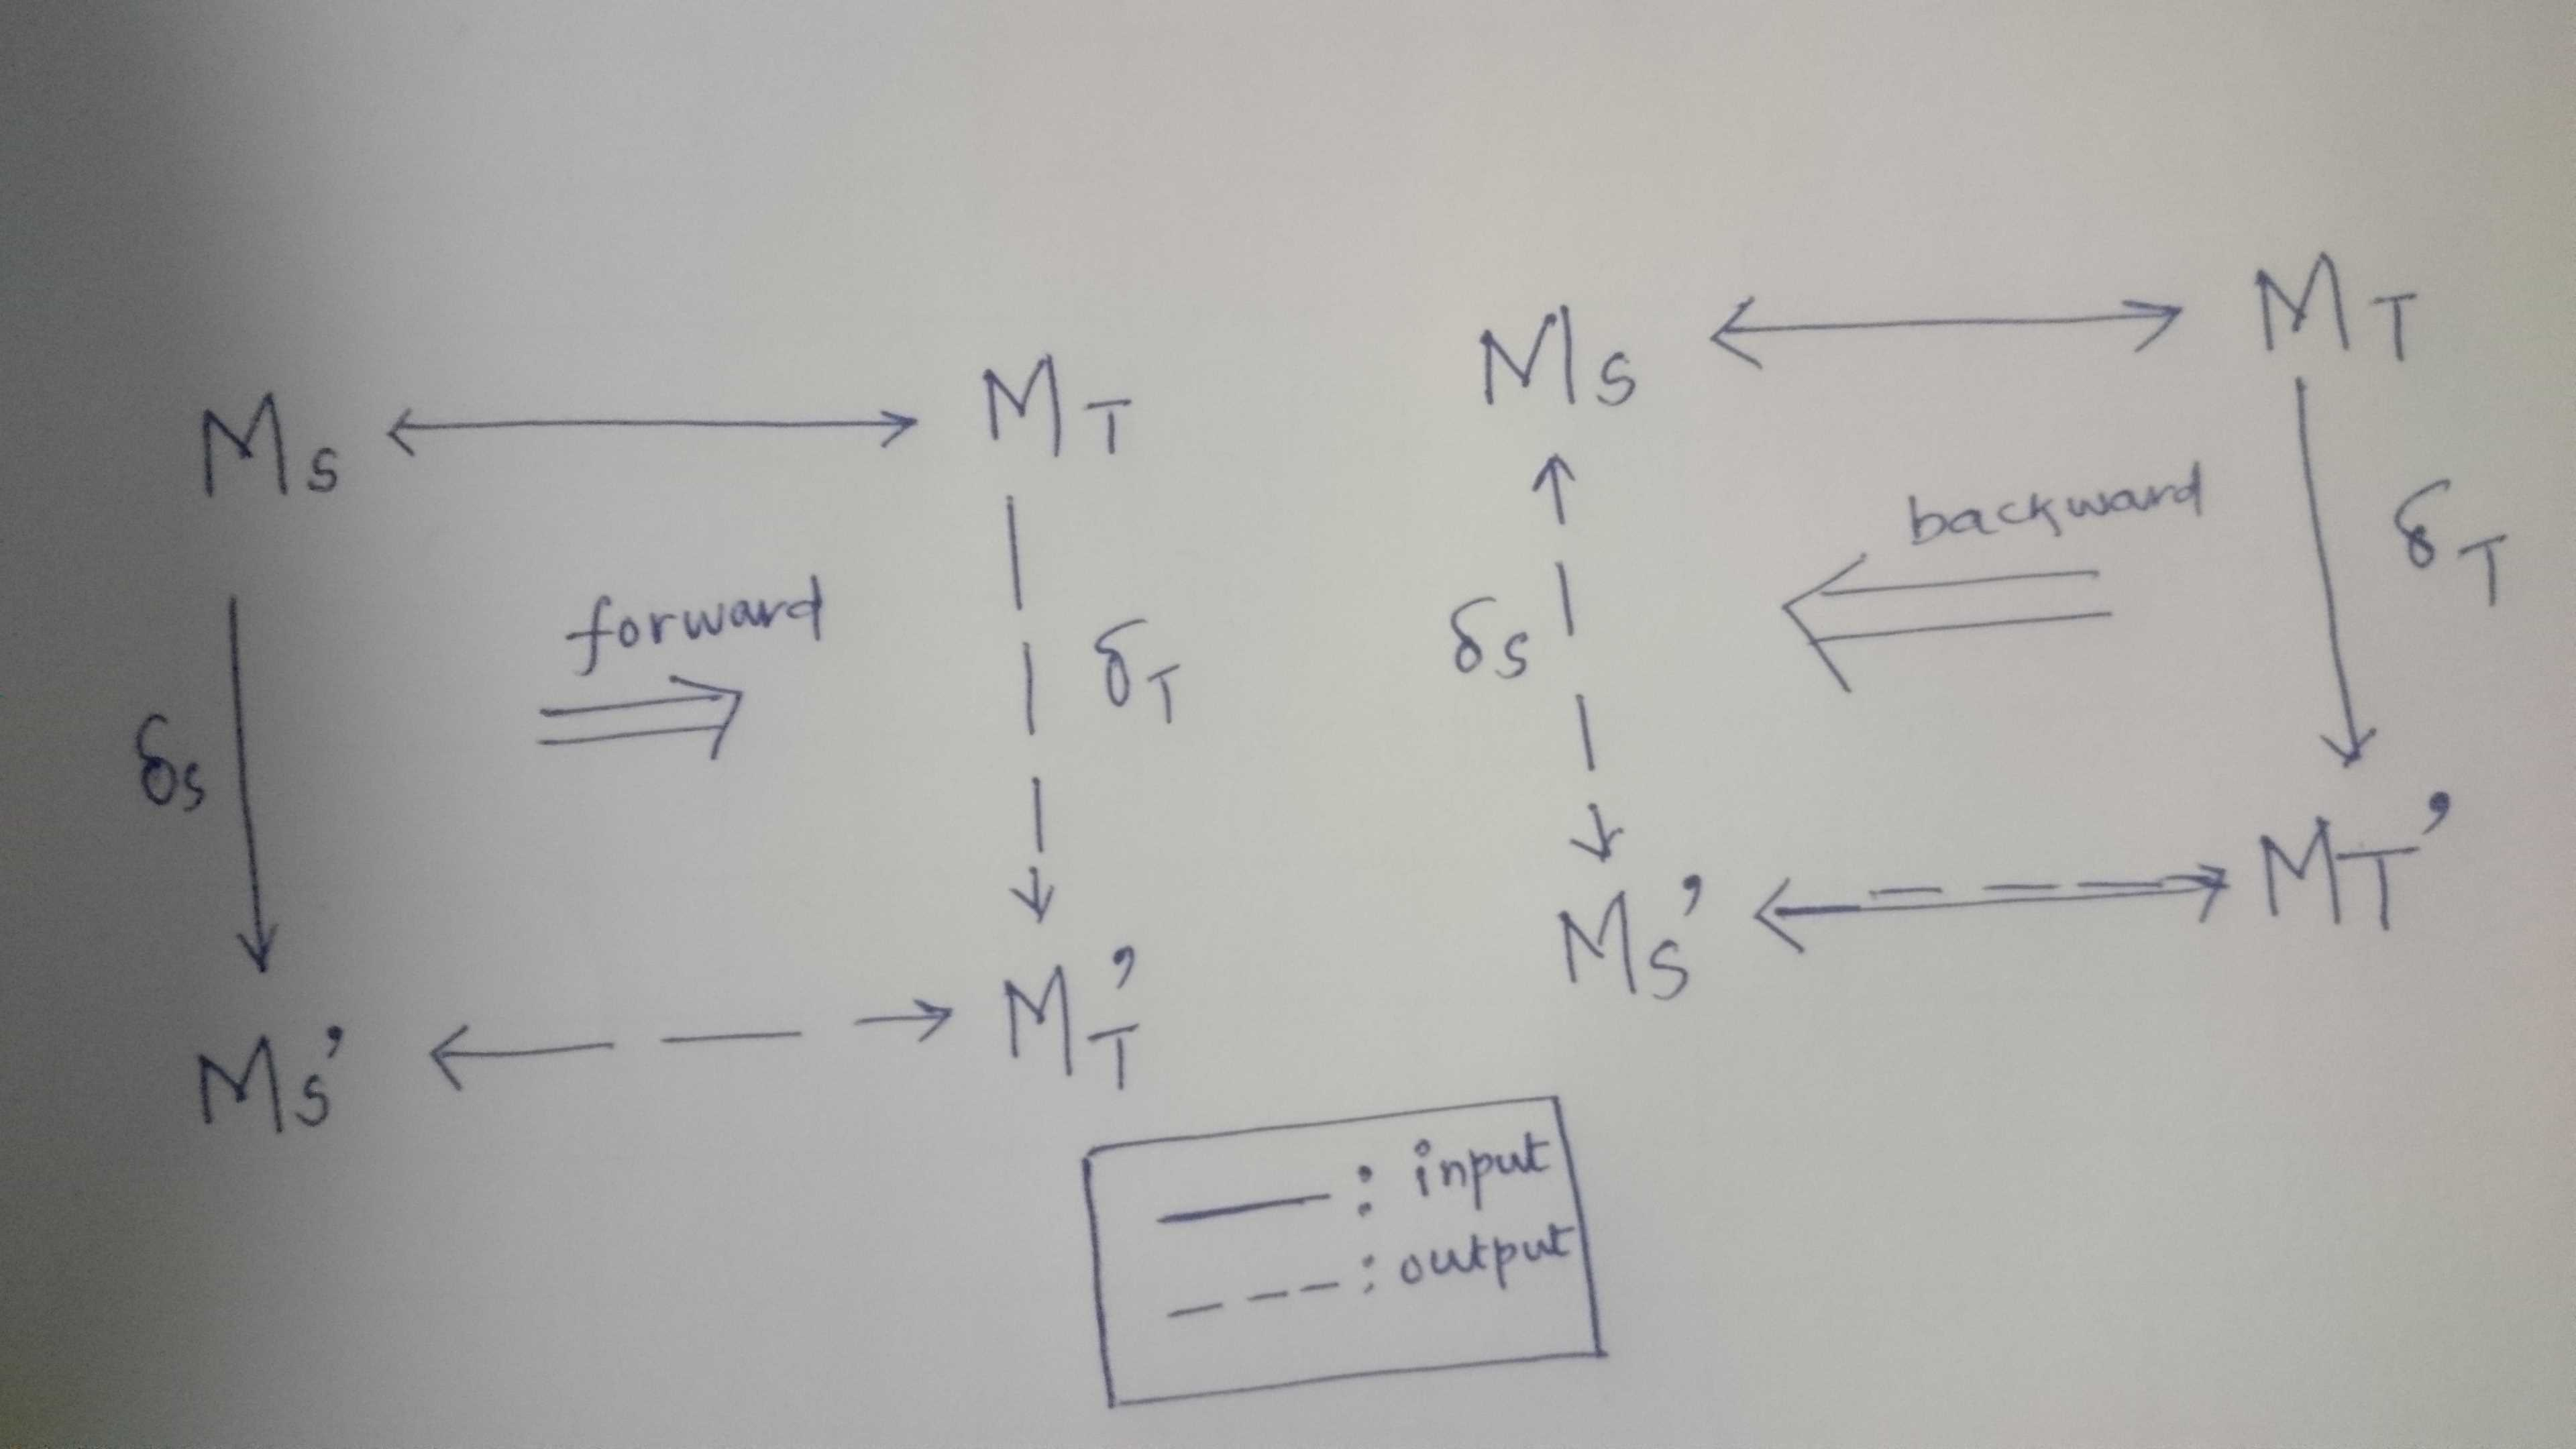
\includegraphics[width=1\textwidth]{figures/BX}
	\caption{Bidirectional Transformation}
	\label{fig:BX_Diagram}
\end{figure}


 



